% Created 2023-08-29 Tue 12:37
% Intended LaTeX compiler: pdflatex
\documentclass[11pt]{article}
\usepackage[utf8]{inputenc}
\usepackage[T1]{fontenc}
\usepackage{graphicx}
\usepackage{longtable}
\usepackage{wrapfig}
\usepackage{rotating}
\usepackage[normalem]{ulem}
\usepackage{amsmath}
\usepackage{amssymb}
\usepackage{capt-of}
\usepackage{hyperref}
\usepackage{array, tikz, pgfplots}
\author{Hankertrix}
\date{\today}
\title{Math Module 1B Lecture Notes}
\hypersetup{
 pdfauthor={Hankertrix},
 pdftitle={Math Module 1B Lecture Notes},
 pdfkeywords={},
 pdfsubject={},
 pdfcreator={Emacs 29.1 (Org mode 9.6.6)}, 
 pdflang={English}}
\begin{document}

\maketitle
\setcounter{tocdepth}{2}
\tableofcontents

\newpage

\section{Limits}
\label{sec:org803a9e2}

\subsection{The idea of limit}
\label{sec:orgbe71e73}

Let \(f(x) = \frac{\sin x}{x}\). What happens to \(f(x)\) of values of \(x\) near 0?

We can observe that:

\begin{center}
\begin{tabular}{c c|c c}
x & f(x) & x & f(x) \\
\hline
0.1 & 0.998 & -0.1 & -0.998 \\
0.01 & 0.99998 & -0.01 & 0.99998 \\
0.001 & 0.9999998 & -0.001 & 0.9999998 \\
0.0001 & 0.999999998 & -0.0001 & 0.999999998
\end{tabular}
\end{center}

It \textbf{looks like} the function values of \(f(x)\) get closer and closer to 1 as \(x\) approaches 0.


\subsection{Plotting approach}
\label{sec:org7bab5ca}

We can plot the graph:
\\[0pt]
\\[0pt]

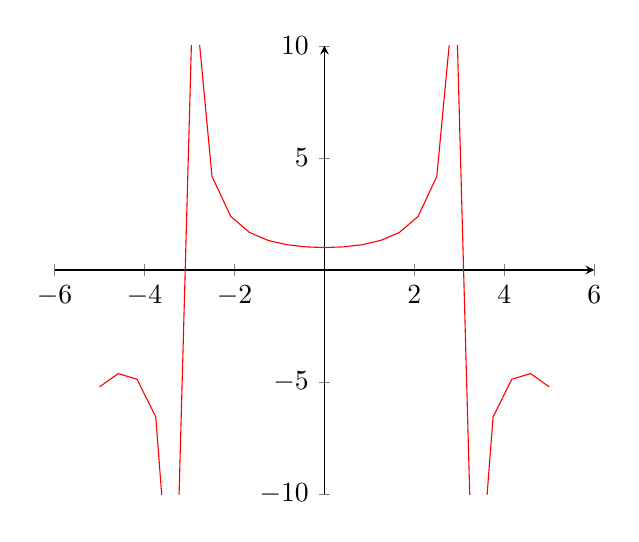
\begin{tikzpicture}
\begin{axis}[axis lines = middle, xmin = -6, xmax = 6, ymin = -10, ymax = 10]
\addplot[color = red]{x / sin(deg(x))};
\end{axis}
\end{tikzpicture}

\newpage

\subsection{Limits, in rigorous terms}
\label{sec:orgfdcef37}
From a maths perspective, "\textbf{looks like}" isn't good enough.
\\[0pt]

But before we can do anything better, we have to \textbf{exactly define} what we're talking about in the first place.
\\[0pt]

Roughly speaking, if \(f(x)\) can be made arbitrarily close to some number \(L\) by taking the value of the variable \(x\) sufficiently close to \(a\), but not equal to \(a\), then we'd like to say that \(L\) is \(f\)'s limit at the point \(a\).
\\[0pt]

In simpler terms, if \(f(x)\) approaches a value \(L\) but isn't equal to \(L\), that means that \(L\) is \(f\)'s limit.


\subsection{Distance between points}
\label{sec:org49d12fc}

\subsubsection{Definition}
\label{sec:org15295e6}
The distance between two points \(x, y \in \mathbb{R}\) is \(|x - y|\).

\subsubsection{Examples}
\label{sec:org0e72403}
The distance between 5 and 7 is \(7 - 5 = 2\).
\\[0pt]

The distance between 7 and 5 is also \(7 - 5 = 2\).


\subsubsection{Thinking in distances}
\label{sec:org3e9849d}

For expressions such as the one below:

\begin{equation*}
|x - a| < \delta, \, (\delta > 0)
\end{equation*}

It is usually helpful to think of these expressions in terms of distances, i.e. "the point \(x\) is within distance \(\delta\) from \(a\)". Note that for \(\delta > 0\):

\begin{equation}
|x - a| < \delta \Leftrightarrow x \in (a - \delta, a + \delta)
\end{equation}

\newpage

\subsection{Limit points}
\label{sec:orga8efeb7}

\subsubsection{Definition}
\label{sec:org4ed76d7}
Let \(A\) be a subset of \(\mathbb{R}\). We say that a point \(a \in \mathbb{R}\) is a \textbf{limit point} of \(A\), if for every \(\delta > 0\), there exists a point \(x \in A\) such that \(0 < |x - a| < \delta\).
\\[0pt]

Basically, this means that \(a\) is a limit point of \(A\) if there is a point \(x\) such that \(0 < |x - a| < \delta\), or that the absolute value of \(x - a\) is between \(0\) and \(\delta\).


\subsubsection{Example 1}
\label{sec:org555ccef}
Consider \(A = (0, 1] \cup {2}\).
\\[0pt]
\\[0pt]

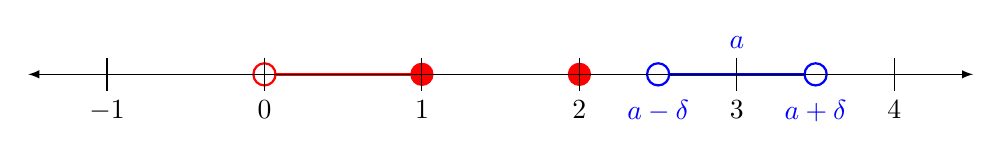
\begin{tikzpicture}[scale = 2]

% The red line representing the range
\draw[color = red, very thick] (0,0) -- (1,0);
\draw[color = blue, very thick] (2.5,0) -- (3.5,0);

% The circles representing the points
\path [draw=red, fill=red] (1,0) circle (2pt);
\path [draw=red, fill=white, thick] (0,0) circle (2pt);
\path [draw=red, fill=red] (2,0) circle (2pt);
\path [draw=blue, fill=white, thick] (2.5,0) circle (2pt);
\path [draw=blue, fill=white, thick] (3.5,0) circle (2pt);

% The number line
\draw[latex-latex] (-1.5,0) -- (4.5,0) ;
\foreach \x in {-1,0,1,2,3,4}
\draw[shift={(\x,0)},color=black] (0pt,3pt) -- (0pt,-3pt);
\foreach \x in {-1,0,1,2,3,4}
\draw[shift={(\x,0)},color=black] (0pt,0pt) -- (0pt,-3pt) node[below]
{$\x$};

% The labels for a and a - δ
\node [below, color=blue] at (2.5,-0.1) {$a - \delta$};
\node [above, color=blue] at (3,0.1) {$a$};
\node [below, color=blue] at (3.5,-0.1) {$a + \delta$};
\end{tikzpicture}
\\[0pt]

Is 3 a limit point of \(A\)?
\\[0pt]

From the definition of the limit point of \(A\), \(a \in \mathbb{R}\) is a limit point of \(a\) if for every \(\delta > 0\), there exists a \(x \in A\) such that \(0 < |x - a| < \delta\).
\\[0pt]

Let \(\delta = \frac{1}{2}\). At \(a = 3\), there does not exist \(x \in A\) such that \(0 < |x - a| < \delta\). Hence, \(a = 3\) is \textbf{not} a limit point of \(A\).

\newpage

\subsubsection{Example 2}
\label{sec:org510e8c6}
Consider \(A = (0, 1] \cup {2}\).
\\[0pt]
\\[0pt]

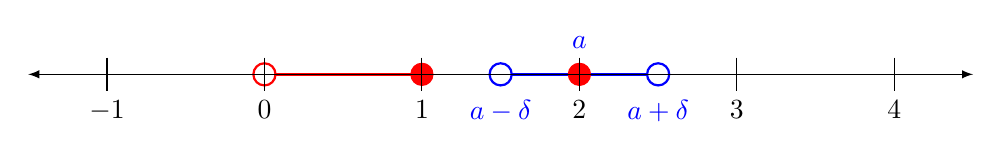
\begin{tikzpicture}[scale = 2]

% The red line representing the range
\draw[color = red, very thick] (0,0) -- (1,0);
\draw[color = blue, very thick] (1.5,0) -- (2.5,0);

% The circles representing the points
\path [draw=red, fill=red] (1,0) circle (2pt);
\path [draw=red, fill=white, thick] (0,0) circle (2pt);
\path [draw=red, fill=red] (2,0) circle (2pt);
\path [draw=blue, fill=white, thick] (1.5,0) circle (2pt);
\path [draw=blue, fill=white, thick] (2.5,0) circle (2pt);

% The number line
\draw[latex-latex] (-1.5,0) -- (4.5,0) ;
\foreach \x in {-1,0,1,2,3,4}
\draw[shift={(\x,0)},color=black] (0pt,3pt) -- (0pt,-3pt);
\foreach \x in {-1,0,1,2,3,4}
\draw[shift={(\x,0)},color=black] (0pt,0pt) -- (0pt,-3pt) node[below]
{$\x$};

% The labels for a and a - δ
\node [below, color=blue] at (1.5,-0.1) {$a - \delta$};
\node [above, color=blue] at (2,0.1) {$a$};
\node [below, color=blue] at (2.5,-0.1) {$a + \delta$};
\end{tikzpicture}
\\[0pt]

Is 2 a limit point of \(A\)?
\\[0pt]

From the definition of the limit point of \(A\), \(a \in \mathbb{R}\) is a limit point of \(a\) if for every \(\delta > 0\), there exists a \(x \in A\) such that \(0 < |x - a| < \delta\).
\\[0pt]

Let \(\delta = \frac{1}{2}\). At \(a = 2\), there does not exist \(x \in A\) such that \(0 < |x - a| < \delta\). Hence, \(a = 2\) is \textbf{not} a limit point of \(A\).


\subsubsection{Example 3}
\label{sec:org2c12dda}
Consider \(A = (0, 1] \cup {2}\).
\\[0pt]
\\[0pt]

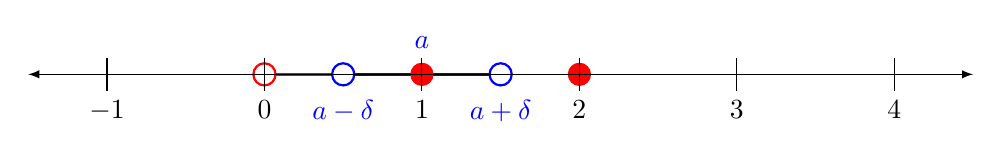
\begin{tikzpicture}[scale = 2]

% The red line representing the range
\draw[color = red, very thick] (0,0) -- (1,0);
\draw[color = blue, very thick] (0.5,0) -- (1.5,0);

% The circles representing the points
\path [draw=red, fill=red] (1,0) circle (2pt);
\path [draw=red, fill=white, thick] (0,0) circle (2pt);
\path [draw=red, fill=red] (2,0) circle (2pt);
\path [draw=blue, fill=white, thick] (0.5,0) circle (2pt);
\path [draw=blue, fill=white, thick] (1.5,0) circle (2pt);

% The number line
\draw[latex-latex] (-1.5,0) -- (4.5,0) ;
\foreach \x in {-1,0,1,2,3,4}
\draw[shift={(\x,0)},color=black] (0pt,3pt) -- (0pt,-3pt);
\foreach \x in {-1,0,1,2,3,4}
\draw[shift={(\x,0)},color=black] (0pt,0pt) -- (0pt,-3pt) node[below]
{$\x$};

% The labels for a and a - δ
\node [below, color=blue] at (0.5,-0.1) {$a - \delta$};
\node [above, color=blue] at (1,0.1) {$a$};
\node [below, color=blue] at (1.5,-0.1) {$a + \delta$};
\end{tikzpicture}
\\[0pt]

Is 1 a limit point of \(A\)?
\\[0pt]

From the definition of the limit point of \(A\), \(a \in \mathbb{R}\) is a limit point of \(a\) if for every \(\delta > 0\), there exists a \(x \in A\) such that \(0 < |x - a| < \delta\).
\\[0pt]

Let \(\delta > 0\). At \(a = 1\), there exists a \(x \in A\) such that \(0 < |x - a| < \delta\). Hence, \(a = 1\) \textbf{is} a limit point of \(A\).
\\[0pt]

\(\frac{1}{2}\) and 0 is also a limit point of \(A\).

\newpage

\subsection{Definition of a limit}
\label{sec:org08a46f0}
For a function \(f: A \rightarrow \mathbb{R}, \, A \subset \mathbb{R}\) with \(a\) as a limit point of \(A\), \(f\) approaches a \textbf{limit} \(L\) if for every \(\varepsilon > 0\), there exists a \(\delta > 0\) such that:

\[\lim_{x \rightarrow a} f(x) = L\]
\[\Updownarrow\]

For every \(\varepsilon > 0\), there exists a \(\delta > 0\) such that:
\[0 < |x - a| < \delta, \quad x \in A \ \ \Rightarrow \ \ |f(x) - L| < \varepsilon.\]

For a visual example, visit this \href{https://www.desmos.com/calculator/fmcqwj1ama}{link}.
\\[0pt]

This \href{https://www.khanacademy.org/math/ap-calculus-ab/ab-limits-new/ab-limits-optional/v/limit-intuition-review}{playlist} should help you understand the definition of a limit if the definition above still doesn't make any sense to you.

\subsubsection{Example 1}
\label{sec:org9452ff1}

Prove that \(\lim_{x \rightarrow 2} \, 17x = 34\).
\\[0pt]

We want to show that for every \(\varepsilon > 0\), there exists \(\delta > 0\), such that:
\[0 < |x - 2| < \delta, \quad x \in \mathbb{R} \ \ \Rightarrow \ \ |17x - 34| < \varepsilon\]

Hence:
\[|17x - 34| = 17|x - 2|\]
\[17|x - 2| < \varepsilon\]
\[|x - 2| < \frac{\varepsilon}{17}\]

Thus, we will need \(\delta = \frac{\varepsilon}{17}\).
\\[0pt]

Let \(\varepsilon > 0\). If we choose \(\delta = \frac{\varepsilon}{17}\), we have:
\[0 < |x - 2| < \delta \ \ \Rightarrow \ \ |17x - 34| = 17|x - 2| < 17\delta = \varepsilon\]

So, by definition,
\[\lim_{x \rightarrow 2} 17x = 34 \textbf{ (Proven)}\]

\newpage

\subsubsection{Example 2}
\label{sec:org8c57d7f}

Prove that \(\lim_{x \rightarrow 0} \, x \sin \frac{1}{x} = 0\).
\\[0pt]

We want to show that for every \(\varepsilon > 0\), there exists a \(\delta > 0\) such that:
\[0 < |x - 0| < \delta, \quad x \in \mathbb{R} \ \ \Rightarrow \ \ \left|x \sin \frac{1}{x} - 0 \right| < \varepsilon\]

Hence:
\[|x \sin \frac{1}{x}| = |x| \cdot |\sin \frac{1}{x}|\]

\begin{align*}
|x| \cdot |\sin \frac{1}{x}| &\leq |x| \\
&< \delta = \varepsilon
\end{align*}

Thus, we will need \(\delta = \varepsilon\).
\\[0pt]

Let \(\varepsilon > 0\). If we choose \(\delta = \varepsilon\), we have:
\begin{align*}
0 < |x - 0| < \delta &\Rightarrow \left|x \sin \frac{1}{x} - 0 \right| \\
&\Rightarrow |x| \cdot \left|\sin \frac{1}{2} \right| \leq |x| < \delta = \varepsilon
\end{align*}

So, by definition,
\[\lim_{x \rightarrow 0} x \sin \frac{1}{x} = 0 \textbf{ (Proven)}\]

\newpage

\subsubsection{Example 3}
\label{sec:org22b7e97}
Prove that \(\lim_{x \rightarrow 2} \, x^2 = 4\).
\\[0pt]

We want to show that for every \(\varepsilon > 0\), there exists a \(\delta > 0\) such that:
\[0 < |x - 2| < \delta, \quad x \in \mathbb{R} \ \ \Rightarrow \ \ |x^2 - 4| < \varepsilon\]

Hence:
\[|x^2 - 4| = |x + 2| \cdot | x - 2| < 5|x - 2|\]
\[5|x - 2| < \varepsilon\]
\[|x - 2| < \frac{\varepsilon}{5}\]

If \(|x - 2| < 1\), then \(x \in (1,3)\), so \(|x + 2| < 5\).
\\[0pt]

Thus, we will need \(\delta = min\{1, \frac{\varepsilon}{5}\} > 0\).

Let \(\varepsilon > 0\). If we choose \(\delta = min\{1, \frac{\varepsilon}{5}\}\), we have:
\[0 < |x - 2| < \delta \quad \Rightarrow \quad |x - 2| < \frac{\varepsilon}{5}\]

And

\begin{align*}
|x - 2| < 1 \quad &\Rightarrow \quad |x^2 - 4| = \begin{aligned}[t]
&|x + 2| \cdot |x - 2| < 5|x - 2| \\
&\because \ |x - 2| < 1 \ \ \text{so} \ \ x \in (1, 3) \\
& \quad \text{and } |x + 2| < 5
\end{aligned} \\
\\
&\Rightarrow \quad |x^2 - 4| < \begin{aligned}[t]
5|x - 2| < \varepsilon \quad \because \ |x - 2| < \frac{\varepsilon}{5}
\end{aligned}
\end{align*}
\\[0pt]

Note that the \(\because\) stands for because.
\\[0pt]

So, by definition:
\[\lim_{x \rightarrow 2} x^2 = 4 \textbf{ (Proven)}\]


\subsubsection{Limits are independent of function values}
\label{sec:org2425974}
It is very important to realise that, given a function \(f(x)\), the value \(f(a)\) does not affect the limit \(\lim_{x \rightarrow a} \, f(x)\). To actually find this limit, we don't need to consider \(f(a)\) and we don't care about whether \(f(a)\) is defined.
\\[0pt]

If there \textbf{exists} a number \(L \in \mathbb{R}\) such that \(\lim_{x \rightarrow a} \, f(x) = L\), we say that \textbf{"f(x) has a limit as \(x\) approaches \(a\)"} or that \textbf{"the limit \(\lim_{x \rightarrow a} \, f(x)\) exists"}.
\\[0pt]

On the contrary, if no such \(L \in \mathbb{R}\) exists, we say that \textbf{"\(f(x)\) has no limit as \(x\) approaches \(a\)"} or that \textbf{"the limit \(\lim_{x \rightarrow a} \, f(x)\) does not exist"}.
\\[0pt]

Note that this has \textbf{nothing to do} with whether or not \(L = 0\). A zero limit is still a limit.

\newpage

\subsection{Limit Laws}
\label{sec:orgd0b800f}

\subsubsection{Theorem}
\label{sec:org2a2f133}
Consider \(f : A_1 \rightarrow \mathbb{R}, g : A_2 \rightarrow \mathbb{R}\). Suppose \(a\) is a limit point of \(A_1 \cap A_2\), and \(\lim_{x \rightarrow a} \, f(x) = l, \lim_{x \rightarrow a} \, g(x) = m\), then:

\begin{align*}
\textbf{1. } \lim_{x \rightarrow a}(Af(x) + Bg(x)) &= Al + Bm \\
&= A \cdot \lim_{x \rightarrow a} f(x) + B \cdot \lim_{x \rightarrow a} g(x)
\end{align*}

\begin{align*}
\textbf{2. } \lim_{x \rightarrow a}(f(x) g(x)) &= lm \\
&= \lim_{x \rightarrow a} f(x) \cdot \lim_{x \rightarrow a} g(x)
\end{align*}

\begin{align*}
\textbf{3. } \lim_{x \rightarrow a} \frac{f(x)}{g(x)} &= \frac{l}{m},
\text{ provided } m \neq 0 \\
&= \frac{\lim_{x \rightarrow a} f(x)}{\lim_{x \rightarrow a} g(x)}
\end{align*}

\begin{align*}
\textbf{4. } \lim_{x \rightarrow a} \sqrt[n]{f(x)} &= \sqrt[n]{l},
\text{ provided } n \in \mathbb{N} \text{ and } l \ge 0 \text{ if } n \text{ is even} \\
&= \sqrt[n]{\lim_{x \rightarrow a} f(x)}
\end{align*}

\textbf{5.} L'H\(\text{\^o}\)pital's rule:
\[\lim_{x \rightarrow a} \frac{f(x)}{g(x)} = \lim_{x \rightarrow a} \frac{f'(x)}{g'(x)}, \text{ when } \lim_{x \rightarrow a} \frac{f(x)}{g(x)} = \frac{0}{0} \text{ and } g'(x) \neq 0\]

\newpage

\subsubsection{Proof of \(\lim_{x \rightarrow a}(Af(x) + Bg(x)) = Al + Bm\)}
\label{sec:org72fd453}

Suppose that:
\[\lim_{x \rightarrow a}f(x) = l, \ \lim_{x \rightarrow a} = m.\]

Let \(\varepsilon > 0\). By our assumptions, there exists a \(\delta_1, \delta_2 > 0\) such that:
\[0 < |x - a| < \delta_1, \ x \in A_1, \quad \Rightarrow \quad |f(x) - l| < \frac{\varepsilon}{2(|A| + 1)},\]
\[0 < |x - a| < \delta_2, \ x \in A_2, \quad \Rightarrow \quad |g(x) -m| < \frac{\varepsilon}{2(|B| + 1)}\]

Let \(\delta = min \{\delta_1, \delta_2\}\). Then:
\[0 < |x - a| < \delta, \ x \in A_1 \cap A_2\]
\[\Downarrow\]
\[0 < |x - a| < \delta_1 \ x \in A_1\]
\[0 < |x - a| < \delta_2 \ x \in A_2\]

\[\Downarrow\]
\begin{align*}
|Af(x) + Bg(x) - (Al + Bm)| &\le |A||f(x) - l| + |B||g(x) -m| \\
&< \frac{\varepsilon}{2} \frac{|A|}{|A| + 1} + \frac{\varepsilon}{2} \frac{|B|}{2|B| + 1} \\
&< \varepsilon
\end{align*}

The proofs for the other laws are also quite similar.

\newpage

\subsubsection{Deriving the limits of polynomials}
\label{sec:org1effe54}

Proving \(\lim_{x \rightarrow a} = a\):
\\[0pt]

For \(\varepsilon > 0\), let \(\delta = \varepsilon\). Then:
\[0 < |x - a| < \delta \Rightarrow |x - a| < \delta = \varepsilon,\]

So, \(\lim_{x \rightarrow a} x = a\).
\\[0pt]

Proving \(\lim_{x \rightarrow a} 1 = 1\):
\\[0pt]

For \(\varepsilon > 0\), let \(\delta = 1\). Then:
\[0 < |x - a| < \delta \Rightarrow |1 - 1| < 0 < \varepsilon,\]

So, \(\lim_{x \rightarrow a} 1 = 1\).
\\[0pt]

Then, using \(\lim_{x \rightarrow a}(Af(x) + Bg(x)) = Al + Bm\) that we just proved, we can conclude that:

\begin{align*}
\lim_{x \rightarrow a} (c_1x + c_0) &= \lim_{x \rightarrow a}(c_1x + c_0 \cdot 1 \\
&= c_1a + c_0
\end{align*}

Also, using \(\lim_{x \rightarrow a} f(x)g(x) = lm\), we can conclude that:

\begin{align*}
\lim_{x \rightarrow a} x^2 &= \lim_{x \rightarrow a} x \cdot x \\
&= a \cdot a \\
&= a^2
\end{align*}

Using \(\lim_{x \rightarrow a}(Af(x) + Bg(x)) = Al + Bm\) again, we can get:
\[\lim_{x \rightarrow a}(c_2 x^2 + c_1 x + c_0) = c_2 a^2 + c_1 a + c_0\]

Repeating this argument, we get that for any \textbf{polynomial \(p(x)\)}:
\[p(x) = c_n x^n + c_{n - 1} x^{n - 1} + \ldots + c_2 x^2 + c_1 x + c_0,\]

We have:
\begin{align*}
\lim_{x \rightarrow a}p(x) &= c_n a^n + c_{n - 1} a^{n-1} + \ldots + c_2 a^2 + c_1 a + c_0) \\
&= p(a)
\end{align*}

This property also holds for some other functions as well, as long as \(a\) is in the domain of the function. A few examples are:
\[\text{1. } \lim_{x \rightarrow a} \sin x = \sin a\]
\[\text{2. } \lim_{x \rightarrow a} \cos x = \cos a\]
\[\text{3. } \lim_{x \rightarrow a}  e^x = e^a\]
\[\text{4. } \lim_{x \rightarrow a}  \ln x = \ln a\]

A function with this property is said to be \textbf{continuous}.

\subsubsection{Reformulated limit laws}
\label{sec:org0c034de}
In each of the laws below, the equation only applies \textbf{if the limit on the right-hand side exists and the expression makes sense}. Otherwise, you cannot directly apply the laws below.

\[\text{1. }\lim_{x \rightarrow a}(Af(x) + Bg(x)) = A \lim_{x \rightarrow a}f(x) + B \lim_{x \rightarrow a} g(x)\]
\[\text{2. } \lim_{x \rightarrow a}(f(x) g(x)) = \lim_{x \rightarrow a} f(x) \cdot \lim_{x \rightarrow a} g(x)\]
\[\text{3. } \lim_{x \rightarrow a} \frac{f(x)}{g(x)} = \frac{\lim_{x \rightarrow a} f(x)}{\lim_{x \rightarrow a} g(x)}\]
\[\text{4. } \lim_{x \rightarrow a} \sqrt[n]{f(x)} = \sqrt[n]{\lim_{x \rightarrow a} f(x)}\]
\[\text{5. } \lim_{x \rightarrow a} \frac{f(x)}{g(x)} = \lim_{x \rightarrow a} \frac{f'(x)}{g'(x)}\]


\newpage

\subsubsection{Example 1}
\label{sec:orgd69f537}

Evaluate \(\lim_{x \rightarrow 2} \frac{x^2 - x - 2}{x - 2}\):

\begin{align*}
\lim_{x \rightarrow 2} \frac{x^2 - x - 2}{x - 2} &\neq \frac{2^2 - 2 - 2}{2 - 2} \\
&\neq \frac{0}{0}
\end{align*}

We cannot apply the limit laws directly, so we divide \(x^2 - x - 2\) by \(x - 2\) using long division, we get:

\begin{align*}
\lim_{x \rightarrow 2} \frac{x^2 - x - 2}{x - 2} &= \lim_{x \rightarrow 2} \frac{(x + 1)(x - 2)}{x - 2} \\
&= \lim_{x \rightarrow 2}(x + 1) \\
&= 2 + 1 \\
&= 3
\end{align*}

\subsubsection{Example 2}
\label{sec:orge017073}
Evaluate \(\lim_{x \rightarrow 1} \frac{\sqrt{2 - x} - 1}{x - 1}\):

\begin{align*}
\lim_{x \rightarrow a} \frac{\sqrt{2 - x} - 1}{x - 1} &\neq \frac{\sqrt{2 - 1} - 1}{1 - 1} \\
&\neq 0
\end{align*}

Once again, we cannot apply the limit laws directly, so we multiply \(\lim_{x \rightarrow 1} \frac{\sqrt{2 - x} - 1}{x - 1}\) by \(\frac{\sqrt{2 - x} + 1}{\sqrt{2 - x} + 1}\)

\begin{align*}
\lim_{x \rightarrow 1} \frac{\sqrt{2 - x} - 1}{x - 1} &= \lim_{x \rightarrow 1} \frac{(\sqrt{2 - x } - 1)(\sqrt{2 - x} + 1)}{(x - 1)(\sqrt{2 - x} + 1)} \\
&= \lim_{x \rightarrow 1} \frac{2 - x - 1}{(x - 1)(\sqrt{2 - x} + 1)} \\
&= \lim_{x \rightarrow 1} \frac{1 - x}{- (1 - x)(\sqrt{2 - x} + 1)} \\
&= \lim_{x \rightarrow 1} \frac{1}{- (\sqrt{2 - x} + 1)} \\
&= -\frac{1}{2}
\end{align*}

\subsubsection{Incorrect example}
\label{sec:org72db836}
\(\indent\) The following is \textbf{wrong}:

\begin{align*}
\lim_{x \rightarrow a} x \cdot \frac{1}{x} &= \lim_{x \rightarrow 0} x \cdot \lim_{x \rightarrow 0} \frac{1}{x} \\
&= 0 \cdot \lim_{x \rightarrow 0} \frac{1}{x} \\
&= 0
\end{align*}

Instead, we should do this:
\begin{align*}
\lim_{x \rightarrow 0} \cdot \frac{1}{x} &= \lim_{x \rightarrow 0} 1 \\
&= 1
\end{align*}


\section{Squeeze Theorem}
\label{sec:org18cef31}
Suppose \(f(x) \leq g(x) \leq h(x)\), for \(x \in I \setminus \{a\}\), where \(I\) is some open interval containing the point \(a\). Then:

\[\lim_{x \rightarrow a} f(x) = \lim_{x \rightarrow a} h(x) = L \quad \Rightarrow \quad \lim_{x \rightarrow a} g(x) = L\]

\newpage

\subsection{Proof}
\label{sec:orgc999caa}

Suppose:
\[f(x) \leq g(x) \leq h(x), \text{ for } x \in I \setminus \{a\} \tag{1}\]
\[\lim_{x \rightarrow a}f(x) = \lim_{x \rightarrow a}h(x) = L \tag{2}\]

Let \(\varepsilon > 0\). Since \(I\) is open and \(a \in I\), there exists a \(\delta_1 > 0\) such that \((a - \delta_1, a + \delta_1) \subset I\). And by using equation \((2)\), there exists a \(\delta_2, \delta_3 > 0\) such that:

\[0 < |x - a| < \delta_2, \ x \in dom \, f \ \Rightarrow \ |f(x) - L| < \varepsilon \ \Rightarrow \ L - \varepsilon < f(x)\]
\[0 < |x - a| < \delta_3, \ x \in dom \, h \ \Rightarrow \ |h(x) - L| < \varepsilon \ \Rightarrow \ h(x) < L + \epsilon\]

Note that \(dom\) represents the \textbf{domain} of the function.
\\[0pt]

Let \(\delta = min \{\delta_1, \delta_2, \delta_3\}\). Using equation \((1)\), we get:
\[0 < |x - a| < \delta\]
\[\Downarrow\]
\[x \in I \setminus \{a\}\]
\[0 < |x - a| < \delta_2\]
\[0 < |x - a| < \delta_3\]
\[\Downarrow\]
\[L - \varepsilon < f(x) \leq g(x) \leq h(x) < L + \varepsilon\]
\[\Downarrow\]
\[|g(x) - L| < \varepsilon\]


\subsection{Another useful result}
\label{sec:org678ca14}
For \(f : A \rightarrow \mathbb{R}\), we have:
\[\lim_{x \rightarrow a} f(x) = L \quad \Leftrightarrow \quad \lim_{x \rightarrow a} |f(x) - L| = 0\]

\subsubsection{Proof}
\label{sec:org483b393}
\[\lim_{x \rightarrow a} f(x) = L\]
\[\Updownarrow\]
\[\begin{aligned} &\text{For every } \varepsilon > 0, \text{ there exists a } \delta > 0 \\
&\text{such that } 0 < |x - a| < \delta, \ x \in A
\end{aligned} \quad \Rightarrow \quad |f(x) - L| < \varepsilon\]
\[\Updownarrow\]
\[\begin{aligned} &\text{For every } \varepsilon > 0, \text{ there exists a } \delta > 0 \\
&\text{such that } 0 < |x - a| < \delta, \ x \in A
\end{aligned} \quad \Rightarrow \quad ||f(x) - L| - 0| < \varepsilon\]
\[\Updownarrow\]
\[\lim_{x \rightarrow a}|f(x) - L| = 0\]


\subsubsection{Example 1}
\label{sec:org93d8956}
Evaluate \(\lim_{x \rightarrow 0} x \sin \frac{1}{x}\) (again):
\\[0pt]

Guess, from the graph or otherwise: \(\lim_{x \rightarrow 0} x \sin \frac{1}{x} = 0\)
\\[0pt]

\textbf{Proof}:
\\[0pt]

Note that:
\[\lim_{x \rightarrow 0} x \sin \frac{1}{x} = 0 \quad \Leftrightarrow \quad \lim_{x \rightarrow 0} \left|x \sin \frac{1}{x} - 0 \right| = 0\]

\[0 \leq \left|x \sin \frac{1}{x} \right| = |x| \left|\sin \frac{1}{x} \right| \leq |x|\]

By the squeeze theorem:
\[\lim_{x \rightarrow 0} \left|x \sin \frac{1}{x} \right| = 0\]

Hence:
\[\lim_{x \rightarrow 0} x \sin \frac{1}{x} = 0\]


\subsubsection{Example 2}
\label{sec:org630aea1}
Evaluate \(\lim_{x \rightarrow 0} e^{\sin(\cot x)} x^4\)
\\[0pt]

Guess, from the graph or otherwise: \(\lim_{x \rightarrow 0} e^{\sin(\cot x)} x^4 = 0\)
\\[0pt]

\textbf{Proof}:
\\[0pt]

By the squeeze theorem,
\[|e^{\sin(\cot x)} x^4 - 0| = e^{\sin(\cot x)} \cdot |x^4|\]

Because the range of \(\sin (\cot x)\) is \(x \in [-1, 1]\), the range of \(e^{\sin (\cot x)}\) will be \(x \in [e^{-1}, e^{1}]\), which is less than \(e\):
\[e^{\sin(\cot x)} \cdot |x^4| \leq e \cdot |x^4|\]
\[e \cdot |x^4| \rightarrow 0 \text{ as } x \rightarrow 0\]

Hence:
\[\lim_{x \rightarrow 0} e^{\sin (\cot x)} x^4 = 0\]


\subsection{A lemma}
\label{sec:orgaa498a2}

For \(0 < x < \frac{\pi}{2}\), we have:
\[x \cos^2 x < \sin x < x\]

If \(f\) and \(g\) are \textbf{even} functions such that \(f(x) < g(x)\), for \(x \in (0, a)\), then we also have:
\[f(x) < g(x), \text{ for } x \in (-a, 0)\]

\newpage

\subsubsection{Proof}
\label{sec:org76fada2}

Suppose \(f\) and \(g\) are even and:
\[f(x) < g(x), \text{ for } x \in (0, a)\]

Then for \(x \in (-a, 0)\), let \(u = x\) so \(u \in (0, a)\). We get:
\[f(x) = f(-u) = f(u) < g(u) = g(-u) = g(x)\]

We showed that \(x \cos^2 x < \sin x < x\) for \(x \in (0, \frac{\pi}{2})\).
\\[0pt]

Since \(x > 0\), we get:
\[\cos^2 x < \frac{\sin x}{x} < 1, \text{ for } x \in (0, \frac{\pi}{2})\]

Since all three expressions above are even functions, the two inequalities extend to \((-\frac{\pi}{2}, 0)\). Hence:
\[\cos^2 x < \frac{\sin x}{x} < 1, \text{ for } x \in (- \frac{\pi}{2}, 0) \cup (0, \frac{\pi}{2})\]


\subsubsection{Example 1}
\label{sec:orgc1bc7cf}
Find \(\lim_{x \rightarrow 0} \sin x\):
\\[0pt]

Using the lemma:
\[\frac{\sin x}{x} < 1, \text{ for } x \in (-\frac{\pi}{2}, 0) \cup (0, \frac{\pi}{2})\]

Note that for \(x \in (-\frac{\pi}{2}, 0) \cup (0, \frac{\pi}{2})\), we have:
\[\left|\frac{\sin x}{x} \right| = \frac{\sin x}{x} < 1 \text{ for } x \in (-\frac{\pi}{2}, 0) \cup (0, \frac{\pi}{2})\]

So for \(x \in (-\frac{\pi}{2}, 0) \cup (0, \frac{\pi}{2})\):
\[0 \leq |\sin x| \leq |x|\]

Because by using the squeeze theorem, \(|\sin x|\) approaches 0 and \(|x|\) approaches 0 when x approaches 0.
\\[0pt]

Hence:
\[\lim_{x \rightarrow 0} \sin x = 0\]


\subsubsection{Example 2}
\label{sec:orga2776c2}
Find \(\lim_{x \rightarrow 0} \cos x\):
\\[0pt]

For \(x \in (-\frac{\pi}{2}, 0) \cup (0, \frac{\pi}{2}), \cos x > 0\), so:
\begin{align*}
\cos x &= |\cos x| \\
&= \sqrt{\cos^2 x} \\
&= \sqrt{1 - \sin^2 x}
\end{align*}

Since \(\sin^2 x \rightarrow 0\) as \(x \rightarrow 0\):
\begin{align*}
\sqrt{1 - \sin^2 x} &\rightarrow \sqrt{1} \\
&\rightarrow 1
\end{align*}

Hence:
\[\lim_{x \rightarrow 0} \cos x = 1\]


\subsubsection{Example 3}
\label{sec:org37b8921}
Find \(\lim_{x \rightarrow 0} \frac{\sin x}{x}\):
\\[0pt]

We showed that:
\[\cos^2 x < \frac{\sin x}{x} < 1 \text{ for } x \in (-\frac{\pi}{2}, 0) \cup (0, \frac{\pi}{2})\]

So \(\lim_{x \rightarrow 0} \frac{\sin x}{x} = 1\)


\section{Limits at infinity}
\label{sec:org4a704e2}
We also want to consider a function's behaviour as \(x\) becomes very large (either positive or negative). For example, it is clear that the values of \(f(x) = 4 - \frac{2}{x}\) can be made arbitrarily close to 4 by choosing \(x\) to be large enough.
\\[0pt]

We can express this by writing:
\[\lim_{x \rightarrow + \infty} 4 - \frac{2}{x} = 4\]


\subsection{Definition}
\label{sec:org2c6f293}
Suppose \(f\) is defined on some interval \((a, \infty)\). We say that \(f(x)\) has a limit \(L\) as \(x\) approaches positive infinity, and write \(\lim_{X \rightarrow + \infty} f(x) = L\), if for every \(\varepsilon > 0\), there exists a number \(R\) such that:
\[x > R \quad \Rightarrow \quad |f(x) - L| < \varepsilon\]

Likewise, for \(f\) defined on some interval \((-\infty, b)\), we say that \(f(x)\) has a limit \(L\) as \(x\) approaches negative infinity, and write \(\lim_{x \rightarrow - \infty} f(x) = L\), if for every \(\varepsilon > 0\), there exists a number \(R\) such that:
\[x < R \quad \Rightarrow \quad |f(x) - L| < \varepsilon\]

Limits at infinity follow the same limit laws as normal limits, so we can use limit laws to conclude that for any \textbf{positive} integer \(n\), we also have:
\[\lim_{x \rightarrow \pm \infty} \frac{1}{x^n} = 0\]

When evaluating a limit at infinity, a common technique is to factor out the highest possible power.

\subsection{Example 1}
\label{sec:orgc8e7fc5}
Show that \(\lim_{x \rightarrow + \infty} = 0\).
\\[0pt]

Let \(\varepsilon > 0\) and \(R = \frac{1}{\varepsilon}\). We get:

\begin{align*}
x > R \Rightarrow \left|\frac{1}{x} - 0 \right| &= \frac{1}{|x|} \\
&= \frac{1}{x} \\
&< \frac{1}{R} = \varepsilon
\end{align*}

\[x > R = \frac{1}{\varepsilon} > 0\]

\newpage

\subsection{Example 2}
\label{sec:org64fc32e}
Show that \(\lim_{x \rightarrow - \infty} = 0\).
\\[0pt]

Let \(\varepsilon > 0\) and \(R = \frac{1}{\varepsilon}\). We get:

\begin{align*}
x < R \Rightarrow \left|\frac{1}{x} - 0 \right| &= \frac{1}{|x|} \\
&= \frac{1}{x} \\
&< \frac{1}{R} = \varepsilon
\end{align*}

\[x < R = \frac{1}{\varepsilon} > 0\]

\subsection{Example 3}
\label{sec:org80d99ed}
Find:
\[\lim_{x \rightarrow + \infty} \frac{x^3 + 4x -5}{7x^3 + 3}\]
\\[0pt]

As \(x \rightarrow + \infty\):
\begin{align*}
\frac{x^3 + 4x - 5}{7x^3 + 3} &=
\frac{x^3 \left(1 + \frac{4}{x^2} - \frac{5}{x^3} \right)}
{x^3 \left( 7 + \frac{3}{x^3}\right)} \\
&= \frac{1 + \frac{4}{x^2} - \frac{5}{x^3}}
{7 + \frac{3}{x^3}} \\
&= \frac{1 + \frac{4(1)}{x^2} - \frac{5(1)}{x^3}}
{7 + \frac{3(1)}{x^3}} \\
&\rightarrow \frac{1}{7} \text{ as } x \rightarrow +\infty
\end{align*}

This is because all terms with \(\frac{1}{x^n}\), where \(n \in \mathbb{Z}^+\), approach 0 when \(x \rightarrow + \infty\).
\\[0pt]

Hence:
\[\lim_{x \rightarrow + \infty} \frac{x^3 + 4x -5}{7x^3 + 3} \rightarrow \frac{1}{7} \text{ as } x \rightarrow +\infty\]

\newpage

\subsection{Incorrect example}
\label{sec:org87eb330}
Find:
\[\lim_{x \rightarrow - \infty} \frac{\sqrt{2x^2 + 1}}{3x - 5}\]

\begin{align*}
\frac{\sqrt{2x^2 + 1}}{3x - 5} &=
\frac{\sqrt{x^2 \left(2 + \frac{1}{x^2}\right)}}{x \left(3 - \frac{5}{x} \right)} \\
&= \frac{\sqrt{x^2} \cdot \sqrt{2 + \frac{1}{x^2}}}{x \left(3 - \frac{5}{x} \right)} \\
&= \frac{|x| \sqrt{2 + \frac{1}{x^2}}}{x \left(3 - \frac{5}{x} \right)} \\
&= \frac{x \sqrt{2 + \frac{1}{x^2}}}{x \left(3 - \frac{5}{x} \right)} \\
&= \frac{\sqrt{2 + \frac{1}{x^2}}}{\left(3 - \frac{5}{x} \right)}
\end{align*}

Since \(\frac{1}{x}\) and \(\frac{5}{x}\) approach 0 when \(x \rightarrow \infty\):
\[\frac{\sqrt{2 + \frac{1}{x^2}}}{\left(3 - \frac{5}{x} \right)} \rightarrow \frac{\sqrt{2}}{3} \text{ as } x \rightarrow -\infty\]

\subsubsection{Explanation of why the example is incorrect}
\label{sec:orgb57e602}

\(\indent\) For \(a \ge 0\):
\[x = \sqrt{a} \quad \Leftrightarrow \quad x^2 = a, \ x \ge 0\]

Hence:
\[x = \sqrt{a^2} \quad \Leftrightarrow \quad x^2 = a^2, \ x \ge 0 \quad \Leftrightarrow \quad x = |a|\]
\[\sqrt{a^2} = |a|\]

For example:
\[\sqrt{(-2)^2} = \sqrt{4} = 2 = |-2|\]

The example automatically assumed that \(\sqrt{x^2}\) is \(x\) without considering what \(x\) will be when approaching the limit, as \(x\) in \(\sqrt{x^2}\) can be either \(x\) or \(-x\).

\subsubsection{Important note}
\label{sec:org45738d2}
Do not write \(\sqrt{a^2} = \pm a\), as it is not correct. The square root is a \textbf{function} of its argument and has \textbf{only one} (non-negative) value.
\\[0pt]

For example, the solutions to the equation \(x^2 = a\) for \(a > 0\) are \(x = \pm \sqrt{a}\). Do not write the solution as \(x = \sqrt{a}\) and claim that \(\sqrt{a}\) has both a positive and negative value.

\subsection{Corrected example}
\label{sec:org6b1fec9}
Find:
\[\lim_{x \rightarrow - \infty} \frac{\sqrt{2x^2 + 1}}{3x - 5}\]

\begin{align*}
\frac{\sqrt{2x^2 + 1}}{3x - 5} &=
\frac{\sqrt{x^2 \left(2 + \frac{1}{x^2}\right)}}{x \left(3 - \frac{5}{x} \right)} \\
&= \frac{\sqrt{x^2} \cdot \sqrt{2 + \frac{1}{x^2}}}{x \left(3 - \frac{5}{x} \right)} \\
&= \frac{|x| \sqrt{2 + \frac{1}{x^2}}}{x \left(3 - \frac{5}{x} \right)}
\end{align*}

For \(x < 0\), \(|x| = -x\):
\begin{align*}
\frac{|x| \sqrt{2 + \frac{1}{x^2}}}{x \left(3 - \frac{5}{x} \right)} &=
\frac{-x \sqrt{2 + \frac{1}{x^2}}}{x \left(3 - \frac{5}{x} \right)} \\
&= \frac{- \sqrt{2 + \frac{1}{x^2}}}{3 - \frac{5}{x}}
\end{align*}

Since \(\frac{1}{x^2}\) and \(\frac{1}{x}\) approach 0 as \(x \rightarrow -\infty\):
\[\frac{- \sqrt{2 + \frac{1}{x^2}}}{3 - \frac{5}{x}} \ \rightarrow \ -\frac{\sqrt{2}}{3} \text{ as } x \rightarrow -\infty\]

Hence:
\[\lim_{x \rightarrow - \infty} \frac{\sqrt{2x^2 + 1}}{3x - 5} \rightarrow -\frac{\sqrt{2}}{3} \text{ as } x \rightarrow -\infty\]


\section{Limit of a sequence}
\label{sec:orgcc4af72}

\subsection{Definition}
\label{sec:org218c9df}
We say that a sequence \((a_n)\) has the limit \(L\) and write \(\lim_{n \rightarrow \infty} a_n = L\), if for every \(\varepsilon > 0\), there exists a number \(N\) such that:
\[n > N \quad \Rightarrow \quad |a_n - L| < \varepsilon\]

The limits of sequences are evaluated with similar methods to other forms of limits.

\newpage

\subsection{Example}
\label{sec:orgae72cb1}
Find:
\[\lim_{n \rightarrow \infty} (\sqrt{n^2 + 2n} - n)\]

\begin{align*}
\sqrt{n^2 + 2n} - n &= \frac{(\sqrt{n^2 + 2n} - n)(\sqrt{n^2 + 2n} + n)}{\sqrt{n^2 + 2n} + n} \\
&= \frac{n^2 + 2n - n^2}{\sqrt{n^2 + 2n} + n} \\
&= \frac{2n}{\sqrt{n^2 + 2n} + n} \\
&= \frac{2n}{\sqrt{n^2 \left( 1 + \frac{2}{n} \right)} + n} \\
&= \frac{2n}{|n| \cdot \sqrt{1 + \frac{2}{n}}}
\end{align*}

Since \(|n| = n\) for \(n > 0\):
\begin{align*}
\frac{2n}{|n| \cdot \sqrt{1 + \frac{2}{n}}} &= \frac{2n}{n \sqrt{1 + \frac{2}{n}} + n} \\
&= \frac{2n}{n (\sqrt{1 + \frac{2}{n}} + 1)} \\
&= \frac{2}{\sqrt{1 + \frac{2}{n}} + 1}
\end{align*}

Since \(\frac{2}{n} \rightarrow 0\) when \(n \rightarrow \infty\):
\begin{align*}
\frac{2}{\sqrt{1 + \frac{2}{n}} + 1} &\rightarrow \frac{2}{\sqrt{1} + 1} \\
&\rightarrow \frac{2}{2} \\
&\rightarrow 1 \text{ when } n \rightarrow \infty
\end{align*}
\end{document}